Ostatni syn i potomek małżeństwa Walentego i Antoniny Głąbów -- Stanisław przyszedł na świat 5 czerwca 1919 r. w Mirowie. 

\begin{figure}[!h]
\begin{center}
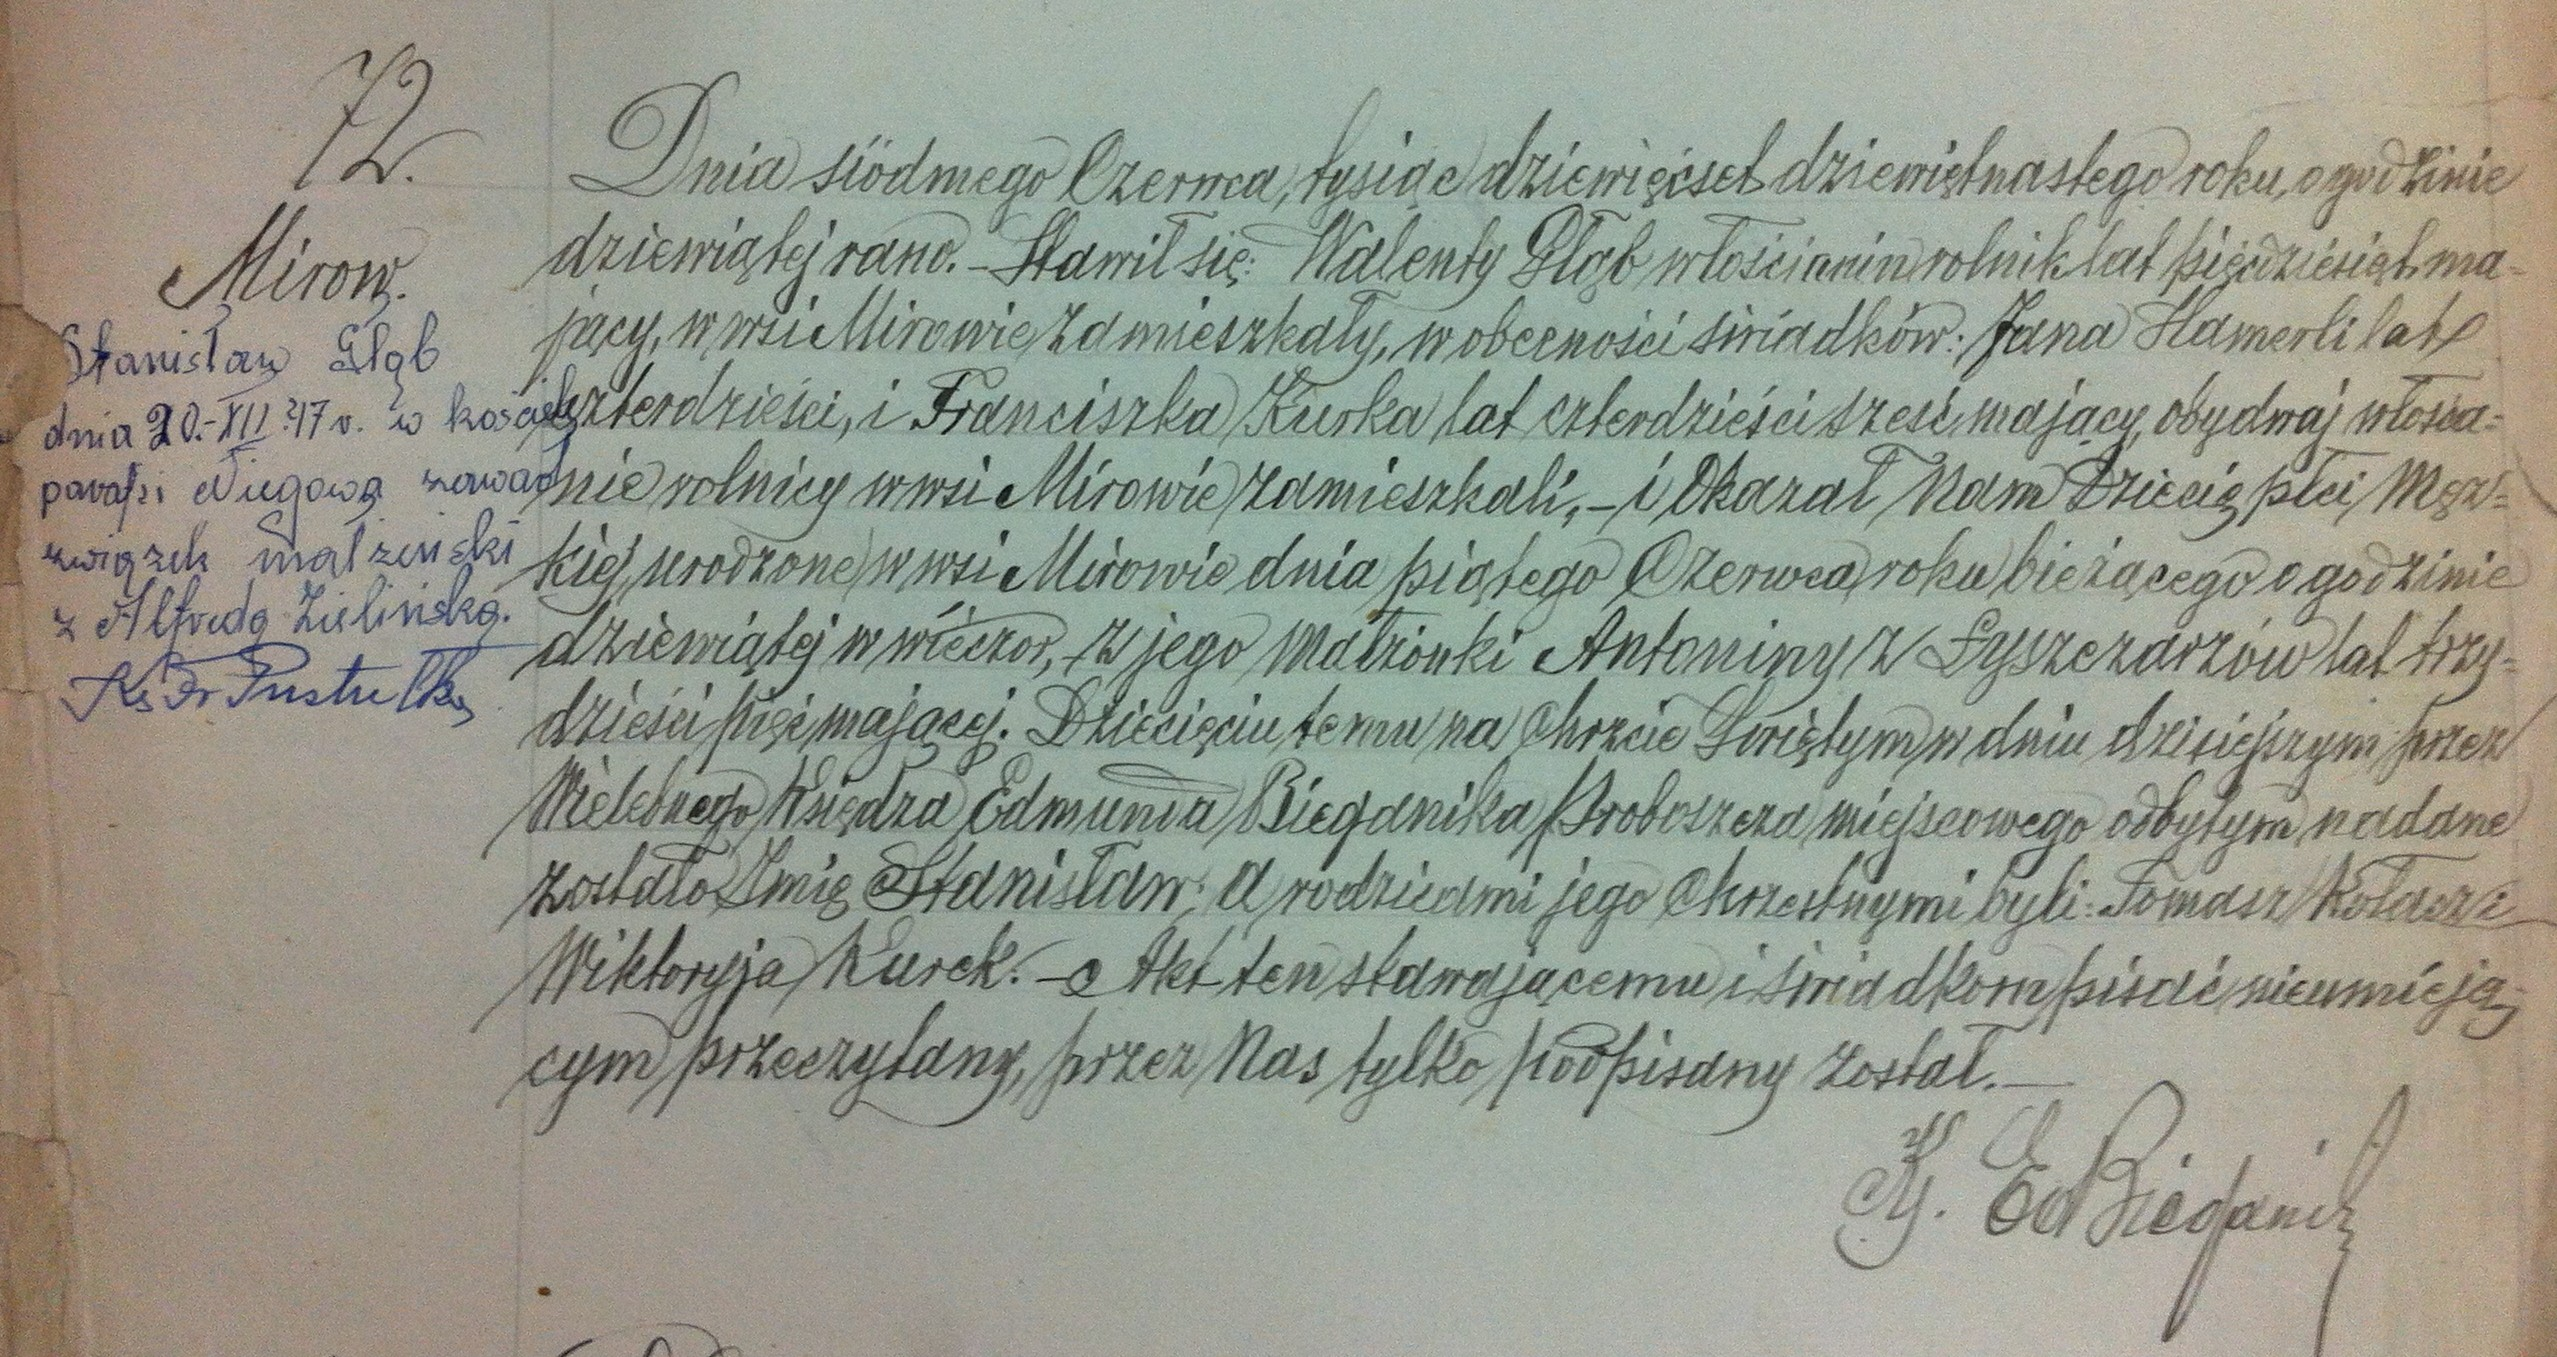
\includegraphics[width=\textwidth]{zdjecia/akt_urodzenia_stanislawa_glaba.jpg}
\caption{Akt urodzenia Stanisława Głąba}
\label{rys:akt_urodzenia_stanislawa_glaba}
\end{center}
\end{figure}


Okazał się on najbardziej utalentowanym technicznie wśród swego rodzeństwa. Ożenił się w Niegowie 20 grudnia 1947 r. (wbrew woli rodziców) z Alfredą Zielińską (ur. 2 X 1928 r. w Mirowie, córką Władysława i Agnieszki ze Szczepańczyków), z którą ma dwie córki: Elżbietę (ur. 15 I 1949 r. w Kopicach koło Grodkowa w woj. opolskim) oraz Dorotę Mariannę (ur. 23 IX 1950 r. w Mirowie). 


\begin{figure}[!ht]
\begin{center}
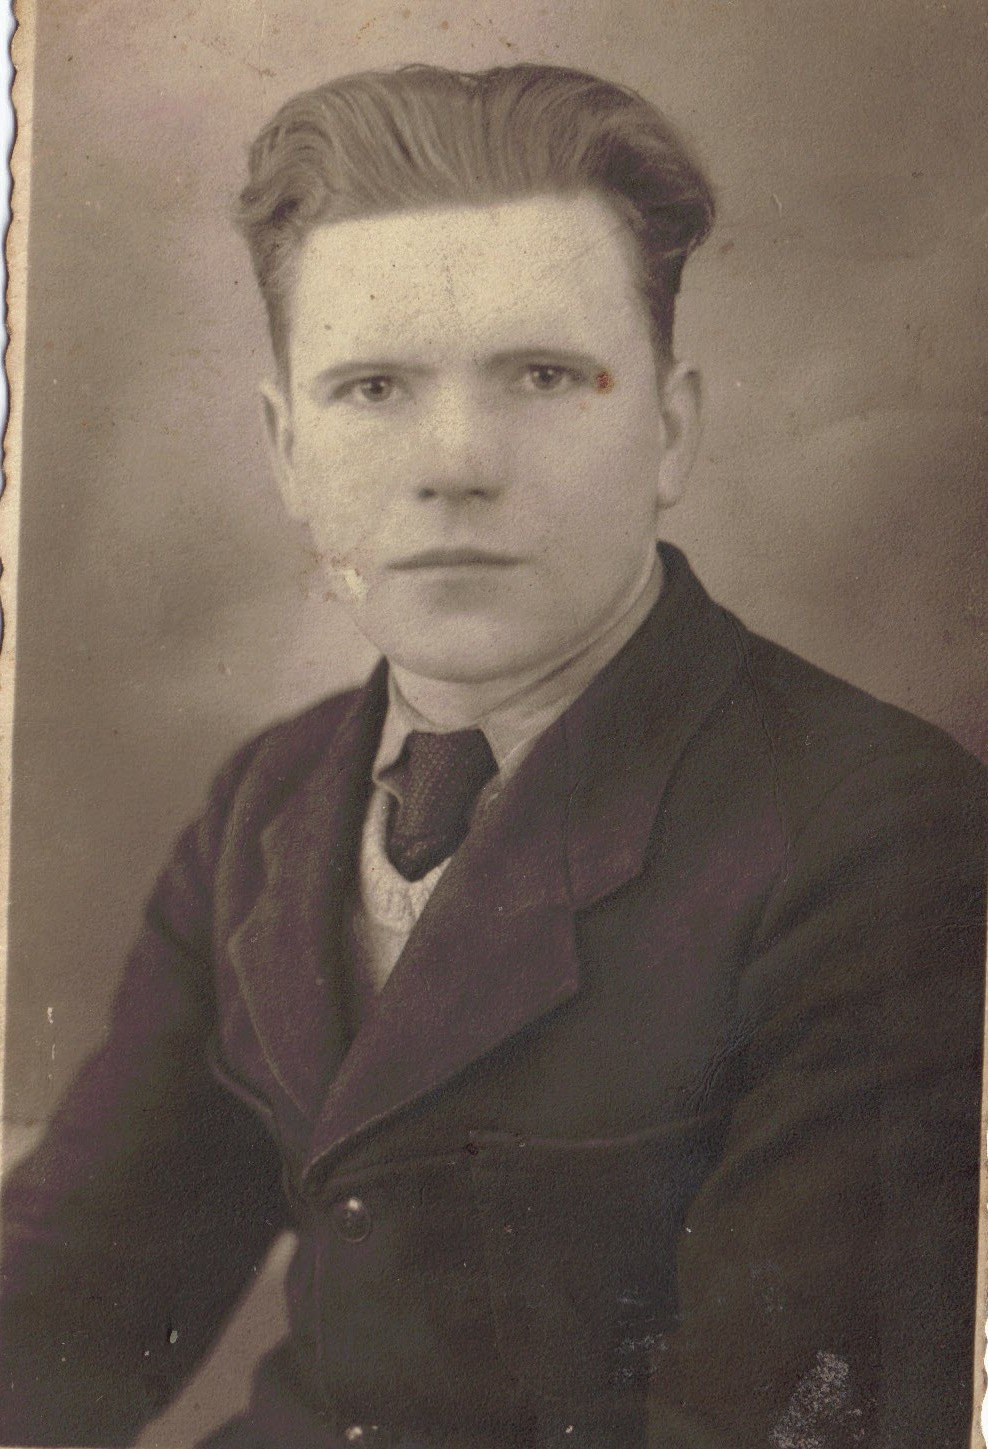
\includegraphics[width=0.45\textwidth]{zdjecia/stanislaw_glab.jpg}
\caption[Stanisław Głąb]{Stanisław Głąb -- syn Walentego i Antoniny}
\label{rys:stanislaw_glab}
\end{center}
\end{figure}

\newpage 
\section{Elżbieta Mostecka z domu Głąb}

Elżbieta wyszła za Zbigniewa Mosteckiego (ur. 4 I 1948r. w Skarżysku Kamiennej), z którym ma dwie córki: Agnieszkę (ur. 21 VIII 1976 r. w Katowicach) i Kamilę (ur. 12 IX 1981 r. w Zawierciu).

Agnieszka wyszła za mąż za Mariusza Stryjka, z którym ma syna Mikołaja, a Kamila wyszła za Marcina Cyzowskiego, z którym ma syna Borysa i córkę Nataszę.




\section{Dorota Podsiadły z domu Głąb}

Dorota wyszła za Adama Podsiadłego, z którym ma córkę Agatę.

Stanisław umarł w 1982 r. w Zawierciu, w wieku 63 lat, a Alfreda w 2009 r. w Zawierciu, w wieku 81 lat.



